\documentclass{article}
\usepackage{pgfplots}
\usepackage{siunitx}
\pgfplotsset{compat=1.18}

\begin{document}

\begin{figure}[h]
\centering
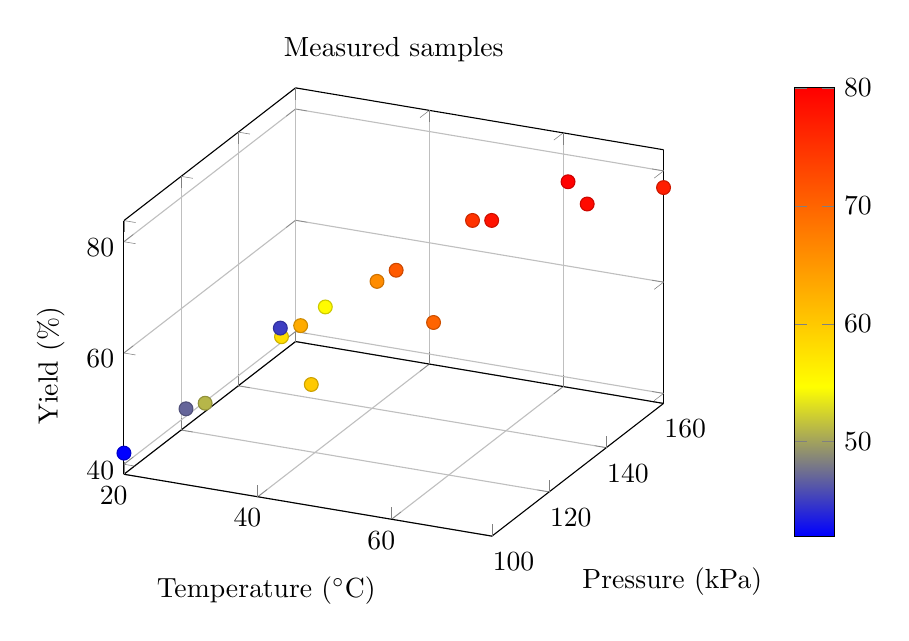
\begin{tikzpicture}
\begin{axis}[
    title={Measured samples},
    xlabel={Temperature (\si{\celsius})},
    ylabel={Pressure (kPa)},
    zlabel={Yield (\%)},
    grid=major,
    colormap/hot,
    colorbar,
]
\addplot3[
    scatter,
    only marks,
    mark=*,
    mark size=2.5pt,
    point meta=z,
] coordinates {
    (20, 100, 42) (25, 110, 47) (30, 105, 51) (35, 120, 58)
    (40, 115, 63) (45, 130, 66) (50, 125, 71) (55, 140, 75)
    (60, 135, 78) (65, 150, 80) (70, 145, 79) (75, 160, 77)
    (22, 150, 45) (33, 140, 55) (48, 100, 60) (62, 110, 70)
};
\end{axis}
\end{tikzpicture}
\caption{Reaction yield as a function of temperature and pressure.}
\end{figure}

\end{document}
